\documentclass{article}
\usepackage{amsmath}
\usepackage{amssymb}
\usepackage{graphicx}
\usepackage{float}
\usepackage{subfig}
\usepackage{hhline}
\usepackage{multirow}
\usepackage{supertabular}
\title{Homework 3}
\date{}
\author{Bastian Haase}
\begin{document}
\maketitle
\tableofcontents
\newpage
\section{Exercise 1}
In this exercise, we want to show that the optimization problem
\begin{align*}
  \min_{p} p^T \nabla f(x) \;\textrm{ subject to } \;\| p \|_{A}=1
\end{align*}
for an SPD matrix $A$ has the solution
$
  p^{*}=-\frac{A^{-1}\nabla f(x)}{\|A^{-1}\nabla f(x) \|_{A}}
$
where we assume $f$ to be smooth.\par
To prove this, we will generalize the proof of the fact that $-\nabla f(x)$ is the direction
of steepest descent. Note that this is the given problem for $A=I$. \par
So, in the spirit of the special case we can see that
\begin{align*}
  p^T \nabla f(x) = p^T A \left( A^{-1} \nabla f(x) \right)=\langle p , A^{-1}\nabla f(x)  \rangle_{A} 
\end{align*}
holds. Here, $\langle \bullet, \bullet \rangle_{A}$ is the inner product induced by $A$. Note that this uses
the assumption that $A$ is SPD. \par
The Cauchy-Schwarz inequality in this setting yields:
\begin{align*}
  \langle p , A^{-1}\nabla f(x)  \rangle_{A} \geq -  \| p \|_{A} \|A^{-1} \nabla f(x) \|_{A}=-\|A^{-1} \nabla f(x) \|_{A}.
\end{align*}
Note that we used the constraint $\| p \|_{A}=1$ in the second step. \par
In view of this inequality, $p^{*}$ is a solution if
\begin{align*}
   \langle p^{*} , A^{-1}\nabla f(x)  \rangle_{A} =-\|A^{-1} \nabla f(x) \|_{A}
\end{align*}
holds. But, this follows easily by using the properties of the inner product:
\begin{align*}
   \langle p^{*} , A^{-1}\nabla f(x)  \rangle_{A}&=\left  \langle -\frac{A^{-1}\nabla f(x)}{\|A^{-1}\nabla f(x) \|_{A}}
, A^{-1} \nabla f(x) \right \rangle_{A}\\
&=-\frac{1}{\|A^{-1}\nabla f(x) \|_{A}} \langle A^{-1}\nabla f(x) , A^{-1}\nabla f(x)  \rangle_{A}\\
&
=-\frac{\|A^{-1}\nabla f(x)\|_{A}^{2}}{\|A^{-1}\nabla f(x) \|_{A}}=-\|A^{-1} \nabla f(x) \|_{A}.
\end{align*}
\section{Exercise 2}
\subsection{Approximating the Action of the Hessian}
In many applications, the Hessian of an objective function is not available or
too costly to compute. In these cases, one can  use methods like
BFGS or steepest descent, but one might wish to still  use Newton methods due
to their local quadratic convergence. An obvious solution to this problem
would be to approximate the action of the Hessian. It is not unreasonable
to hope that a good approximation of the Hessian used in Newton methods will perform similarly to
real Newton methods at least locally. \par
So, given an objective function $f$ and its Jacobian, how can we approximate
the Hessian? One possible way is of course to use Taylor's formula. Given $f$ and its Jacobian, we could either look at the second Taylor polynomial of $f$ or
the first one of $\nabla f$. They are given by the equations
\begin{align}
  f(x+p)&=f(x) +\nabla f(x)p +p^{T} \nabla^{2} f(x) p + \mathcal{O}(\|p\|^{3}) \\
\nabla f(x+p) & = \nabla f(x) + \nabla^{2}f(x)p+\mathcal{O}(\|p\|^{2}).
\end{align}
So, while the first equation gives us a higher accuracy, it has the disadvantage
that we do not approximate the action of the Hessian but just the expression $p^{T} \nabla^{2} f(x) p$. 
However, we can still approximate the Hessian by choosing specific $p$ and solving a linear system of equations.
Let us demonstrate this in the case where $x\in \mathbb{R}^{2}$. Then, the Hessian has the form $\begin{pmatrix}a & b \\ b & d\end{pmatrix}$. Let $e_{i}$ denote
the standard basis vectors. Then, it is straightforward to see that
plugging in $e_1,e_2$ and $e_{1}+e_{2}$ in the expression $p^{T} \nabla^{2} f(x) p$ gives the equations
\begin{align*}
  a&=k  \\
  d&=l  \\
  a+2b+d&=m 
\end{align*}
for some constants $k,l,m \in \mathbb{R}$ dependent on $f$. As this system is,
even numerically, easy to solve, this will give us an approximation of the hessian as we can approximate $k,l$ and $m$. However, note that this system
becomes far more complicated as the dimension increases. \par
The second formula has a lower order of accuracy, but it gives us a direct approximation of the action of the Hessian and is therefore less costly. Also, in order to approximate the Hessian, it is enough to approximate the action on the
standard basis without solving a system of linear equations.\par
In this work, we have decided to use the second formula to approximate the Hessian as the system of equations that we would need to solve when using the first formula would be large for exercise 3. To improve our approximation, we will introduce a \emph{scaling parameter} $\epsilon>0$. Plugging in $\epsilon$ in our approximation, isolating the action of the Hessian and then dividing by $\epsilon$ yields
\begin{align*}
  \nabla^{2} f(x)p\approx\frac{\nabla f(x+\epsilon p)-\nabla f(x)}{\epsilon}
\end{align*}
where  the scaling factor is introduced to take into consideration that
Taylor approximation is more accurate around the center $x$. \par
An implementation of this approximation can be found in \emph{approxHessian.jl}.
We have tested our implementation for the Rosenbrock function
\begin{align*}
  f(x)=(1-x_1)^2+100(x_2-x_1^2)^2
\end{align*}
for $x^{1}=(0,0)$ and $x^{2}=(-1.2,2.5)$. We have chosen six random vectors $p$
of norm 1 and computed the error of our approximation of the action of the Hessian at $x$ on $p$ for various $\epsilon$. The following Figure \ref{action}
visualizes the results.
\begin{figure}[H]
  \centerline{
  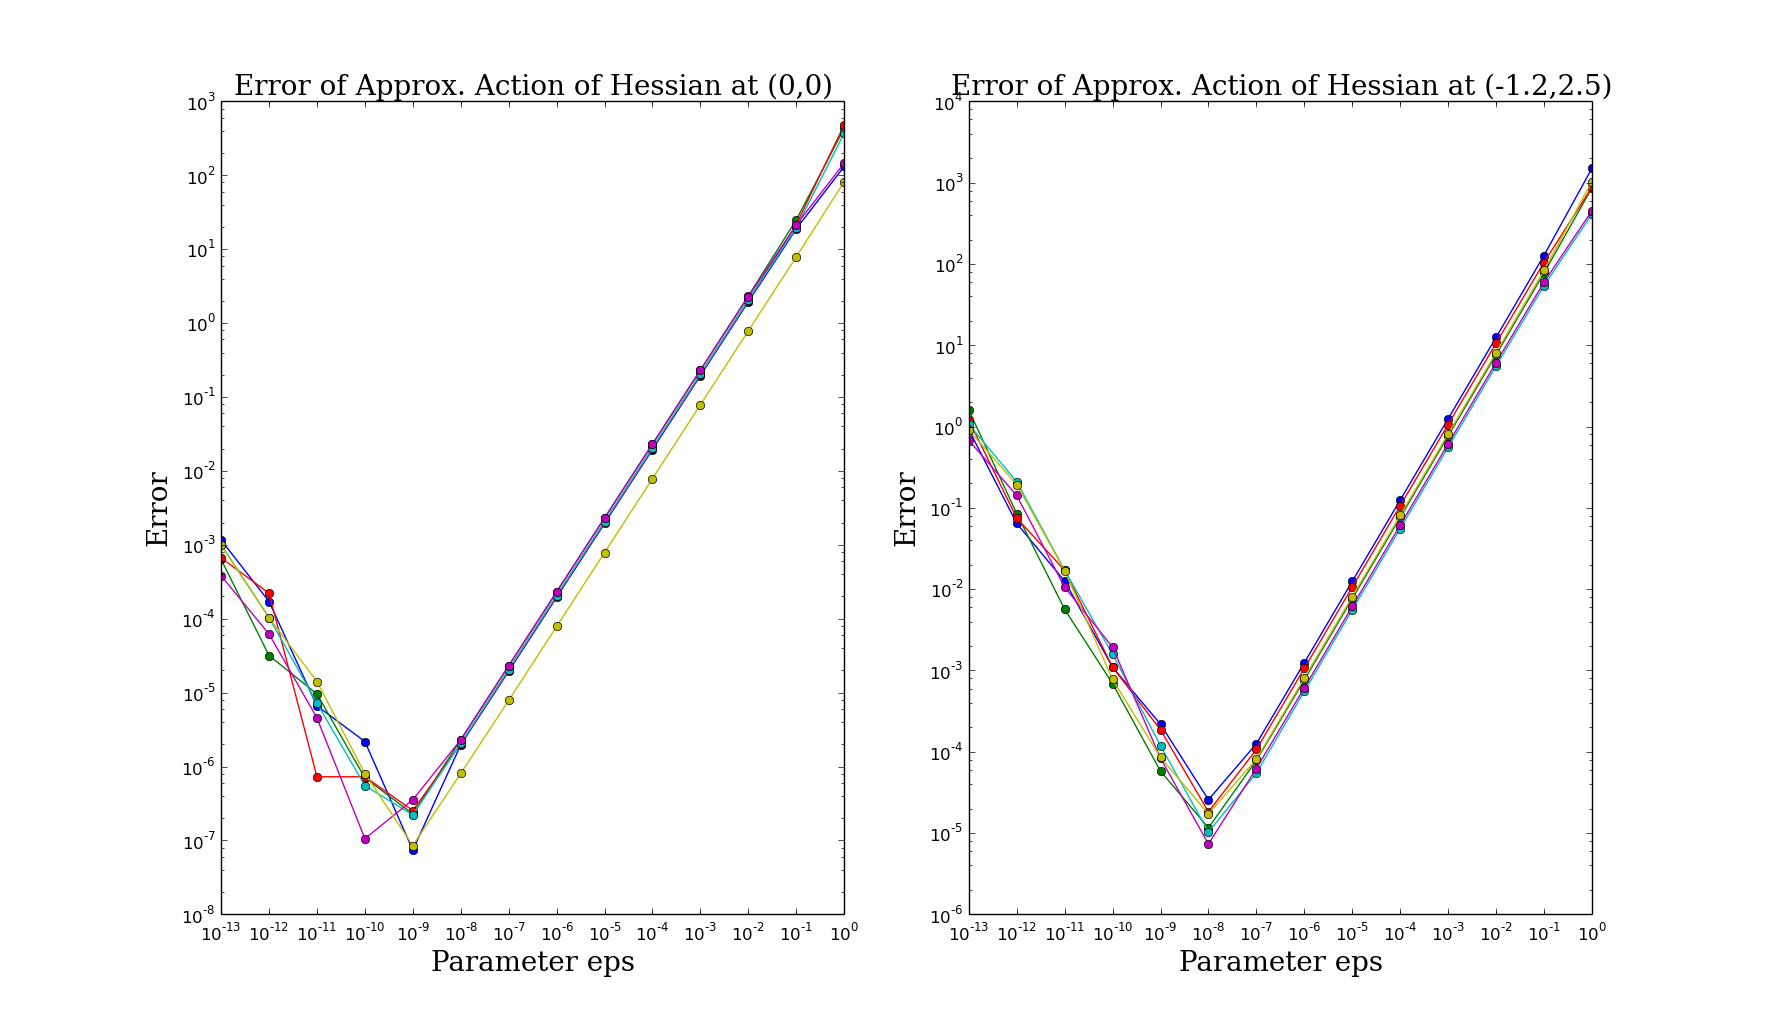
\includegraphics[scale=0.3]{action.png}
  }
  \caption{Error of Approximating Hessian}
\label{action}
\end{figure}
As you can see from the figure, the accuracy of the approximation is comparable
for all directions $p$. The approximation at $x^1=(0,0)$ is more accurate by a factor of  roughly $10^{-2}$ independent of $\epsilon$. This can be, at least partially, explained by comparing the norm of the Hessian at the two points in regards of Taylor's inequality. For $x^1$, the norm is $200$ and for $x^2$ it is approximately $1013$. \par
Maybe the most interesting observation of these graphs is the fact that for very small $\delta$
the approximation becomes very bad. For $\epsilon \geq 10^{-8}$, the change of accuracy with respect to $\epsilon$ is on par with what we expect from Taylor's inequality. But, the bad accuracy for smaller $\epsilon$ contradicts the theory. This phenomenon is most likely caused by the division of $\epsilon$ in our formula and limited machine precision.

\subsection{Minimizing the Rosenbrock Function}
We have minimized the Rosenbrock function with BFGS and NewtonCG methods and starting value
$x_{0}=(-1.2,2.5)$. We stopped our approximation in all cases when the norm of the Jacobian
was below $10^{-8}$. In every method, a standard line search with backtracking and
starting step size 1 was used. \par
We have tested three versions of NewtonCG, the first one, \emph{NewtonCG-H}, being the traditional NewtonCG with the actual Hessian. The second method, \emph{NewtonCG-AH}, uses an approximated Hessian obtained via the procedure described in the last
subsection and parameter $\epsilon=10^{-6}$ as this parameter appears to be a safe choice based on the results obtained. The tests show that it has a high accuracy and is too big to introduce errors caused by limited machine precision. Thirdly, we have used a  NewtonCG variant (\emph{NewtonCG-AA})  where we approximate the action of the
Hessian each time we need it in the conjugate gradient method. The difference between the  last  two versions is that the first one guarantees us a fixed number of Jacobian evaluations per iteration to approximate the Hessian,
namely twice the dimension of $x$. The trade-off is that we have matrix vector multiplications.
The second method avoids these but needs two Jacobian evaluations per CG step. Depending on
the dimension of $x$ and the number of CG steps one or the other method might be preferable.
We have tested them against
a standard implementation of BFGS. \par
As all methods use a steepest descent step in case that we can not compute a search direction (NewtonCG)
or in the case that we can not improve our approximation of the inverse of the Hessian (BFGS) we are
guaranteed global convergence.\par
The following table describes the performance of the methods.
\begin{table}[H]
  \centering
  \begin{tabular}{|l|c|c|c|}
    \hline
   \textbf{Method} & \textbf{Iterations} & \textbf{Fnc. Eval.} &\textbf{Jac. Eval.} \\ \hline
  BFGS &41 &102 &42 \\ \hline
  NewtonCG-H &27 &61 &27 \\ \hline
  NewtonCG-AH&26 &59 &130 \\ \hline
  NewtonCG-AA&27 &62 &131 \\ \hline
 \textbf{Method} & \textbf{Hessian Eval.} & \textbf{Matrix Vect Mult} & \textbf{Matrix Mult.} \\ \hline
   BFGS &0 &41 & 82\\ \hline
   NewotnCG-H &27 &51 &0 \\ \hline
   NewtonCG-AH &0 &50 &0 \\ \hline
   NewtonCG-AA &0 &0 &0 \\ \hline
  \end{tabular}
  \caption{Performance Comparison, Rosenbrock, $x_{0}=(-1.2,2.5)$}
  \label{tab:perform2}
\end{table}
It is noteworthy that all NewtonCG methods have a similar number of iterations. This suggests
that, in this case, our approximation of the Hessian is accurate enough. While the methods
with an approximated Hessian have the advantage of not evaluation the Hessian and no matrix
multiplications, the standard NewtonCG method has fewer function evaluations. If, like in this case, the number of iterations is similar, the approximated versions will be preferable whenever
the Hessian is costly to compute and the dimension of the problem is high. Between the two approximations, the one that approximates the actions performs better as it avoids matrix vector multiplications. While this could potentially be paid for by more Jacobian  evaluations, the low number
of CG steps ($\leq 2$) in this example hides this effect. \par
Comparing BFGS to all three Newton methods we remark that the number of iterations is significantly higher for BFGS. As BFGS converges super-linearly and Newton converges locally quadratic this
result is on line with our expectations. The update also requires a high number of function evaluations and matrix multiplications. Therefore, in this case, Newton methods perform better.\par
For all methods the computation time and memory consumption was recorded and displayed in Table 2.
\begin{table}[H]
  \centering
  \begin{tabular}{|l|c|c|}
    \hline
   \textbf{Method} & \textbf{Time} in sec & \textbf{Memory} in bytes \\ \hline
  BFGS &$4.4e^{-3}$ &$214696$  \\ \hline
  NewtonCG-H &$2.6e^{-4}$ &$88272$  \\ \hline
  NewtonCG-AH&$1.0e^{-2}$ &$353172$  \\ \hline
  NewtonCG-AH2&$3.5e^{-3}$ &$ 124584$\\ \hline
  NewtonCG-AA&$5.4e^{-3}$ &$100352$  \\ \hline
  \end{tabular}
  \label{time1}
  \caption{Time/Memory Comparison, Rosenbrock, $x_{0}=(-1.2,2.5)$}
\end{table}
Here, we have implemented NetwonCG-AH in two ways, where NewtonCG-AH2 is implemented more
directly to avoid any unnecessary memory consumption caused by implementation. In paricular, returning the Hessian through a function is avoided. As we can see, this improves time and
memory consumption a lot and shows us that, in this case, approximating the Hessian or its
action performs similarly. In the next example, we will not be able to use the second implementation due to its high dimension which will make the comparison harder. \par
As computing the Hessian is not costly in this example it is not surprising that the exact NewtonCG-H performs best. Also, higher memory consumption of the BFGS method is not surprising
considering that the BFGS update requires more memory when updating the inverse of the Hessian.
\section{Exercise 3}
Consider the discrete optimal control problem
\begin{align*}
  \min_{u} f(u)=\int_{0}^{T}\; L(y(t),u(t),t)\; dt
\end{align*}
where the state variable $y$ satisfies the ODE
\begin{align*}
  \partial y(t)=F(y(t),u(t),t)
\end{align*}
 given by
\begin{align*}
  L(y,u,t)=(y-3)^2+\frac{1}{2}u^2 \; \textrm{ and } \; F(y,u,t)=uy+t^2
\end{align*}
with $T=1$ and $y_0=0$. In this exercise, we will discretize the problem using forward
Euler, and then approximate a solution using BFGS and NewtonCG with approximated Hessian. \par
Following our discussion in class, if we discretize the problem, then for $\boldsymbol{u} \in \mathbb{R}^{N}$ we get
\begin{align*}
  f(\boldsymbol{u})=(\boldsymbol{y}-3)^2+\frac{1}{2}\boldsymbol{u}^{2}
\end{align*}
Here, $h=T/(N-1)$ denotes the step size and we compute $\boldsymbol{y}$ via forward Euler:
\begin{align*}
  y_{j+1}=y_{j}+h(u_{j}y_{j}+j^2h^2)\;\;\;\; y_{0}=0.
\end{align*}
The adjoint $\boldsymbol{p}$ can be calculated via
\begin{align*}
  p_{j-1}=p_{j}+h(p_{j}u_{j}+2(y_{j}-3)) \; \;\;\; p_{N}=0.
\end{align*}
The implementation of this can be found in \emph{hw3\_ex3.jl}.\par
The derivative can be computed by means of $h,\boldsymbol{u},\boldsymbol{y}$ and $\boldsymbol{p}$
and the formula
\begin{align*}
  \nabla f(x)_{j}=h \left( p_{j} y_{j}+u_{j}  \right)
\end{align*}
which follows from the general description derived in class. The following Figure \ref{deriv}
shows us that the first Taylor polynomial  approximates the
function quadratically, so our derivative seems to be correct.
\begin{figure}[H]
  \centering
  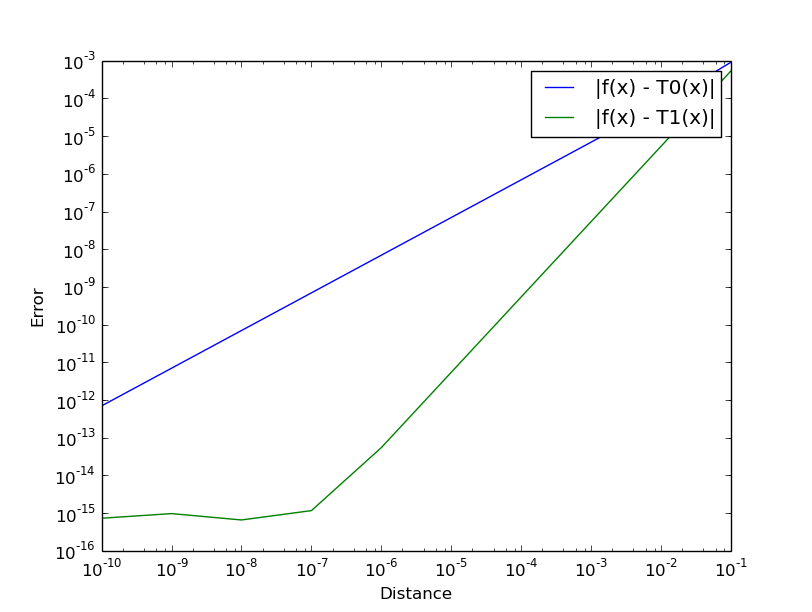
\includegraphics[scale=0.35]{deriv.png}
  \caption{Checking the Derivative}
\label{deriv}
\end{figure}
\subsection{Numerical Stability}
As we us a forward Euler method, we should discuss absolute stability. A method is absolutely stable for a given step size $h$ and a given ODE if the error due to a perturbation of size $\delta$ in
$y_n$ is no larger than  $\delta$ in all $y_m$ for $m>n$. For the ODE of $y$, one can derive the following equation for $z_{j}=y_{j}+\delta$:
\begin{align*}
  z_{j+1}=y_{j}+\delta+hu_{j}(y_{j}+\delta)+t^2=(1+hu_{j})\delta+y_{j+1}.
\end{align*}
So, to guarantee numerical stability, we need $|1+hu_{j}|<1$, the same condition can be derived
for the ODE involving $\boldsymbol{p}$. Unfortunately, as one can see in Figure \ref{final}, $u_{j}$ will
often be positive, so this condition will not be satisfied. However, our methods still converged
to a solution, so the perturbation seems to not have been big enough.
\subsection{Performance of BFGS and Newton}
As we do not know the Hessian of the objective function, we did not apply NewtonCG-H.
But, we  have applied BFGS, NewtonCG-AH and NewtonCG-AA to the described problem for $N=400$ with starting guesses
$u_{0}=10$ and $u_{0}=5+300 \sin(20\pi t)$ until the gradient had a norm smaller than $10^{-8}$. We used standard line search within all three methods with start step size 1. NewtonCG-AH2 could not be implement due to the high dimension of the problem. So, based on the results obtained in section 2,
we should not overemphasize time and memory consumption of NewtonCG-AH as this could be an implementation issue. We have checked that, in  all 6 cases, the method converges to the same solution
as the final state was within a range of $4e^{-6}$ (cmp. \textit{hw3\_ex3.jl}). The following table lists the performance of all methods for both start points.
\begin{table}[H]
  \centering
  \begin{tabular}{|l|c|c|c|}
    \hline
   \textbf{Method} & \textbf{Iterations} & \textbf{Fnc. Eval.} &\textbf{Jac. Eval.} \\ \hline
  BFGS &48 &100 &49 \\ \hline
  NewtonCG-AH&9 &17 &7209 \\ \hline
  NewtonCG-AA&9 &17 &43 \\ \hline
 \textbf{Method} & \textbf{Hessian Eval.} & \textbf{Matrix Vect Mult} & \textbf{Matrix Mult} \\ \hline
    BFGS &0 & 48 & 96 \\ \hline
   NewtonCG-AH &0 &17 &0 \\ \hline
   NewtonCG-AA &0 &0 &0 \\ \hline
  \end{tabular}
  \caption{Performance Comparison, Optimal Control, $u_{0}=10$}
  \label{tab:perform2}
  \begin{tabular}{|l|c|c|c|}
    \hline
   \textbf{Method} & \textbf{Iterations} & \textbf{Fnc. Eval.} &\textbf{Jac. Eval.} \\ \hline
  BFGS &44 &113 &45 \\ \hline
  NewtonCG-AH&6 &12 &4806 \\ \hline
  NewtonCG-AA&6 &12 &30 \\ \hline
 \textbf{Method} & \textbf{Hessian Eval.} & \textbf{Matrix Vect Mult} & \textbf{Matrix Mult} \\ \hline
    BFGS &0 & 44 & 88 \\ \hline
   NewtonCG-AH &0 &12 &0 \\ \hline
   NewtonCG-AA &0 &0 &0 \\ \hline
  \end{tabular}
  \caption{Performance Comparison, Optimal Control, $u_{0}=5 + 300 \sin(20\pi t).$}
  \label{tab:perform3}
\end{table}
We can see that all methods perform better for the second starting value. As the characteristic
of the second starting point are more on par with the final state than the first starting point
(cmp. Figure \ref{final}), this seems plausible. Similar to the last example, NewtonCG-AH and
NewtonCG-AA show comparable values except for the number of function evaluations. This can be 
explained by noting that the number of CG steps ($\leq 3$)  per iteration is much less than the dimension (400). BFGS has more iterations and matrix multiplications with matrices and vectors. Overall,
NewtonCG-AA seems to be the clear winner.
\begin{table}[H]
  \centering
  \begin{tabular}{|l|c|r|}
    \hline
   \textbf{Method} & \textbf{Time} in sec & \textbf{Memory} in bytes \\ \hline
  BFGS &$1.9e^{0}$ &$865494120$  \\ \hline
  NewtonCG-AH&$4.9e^{0}$ &$1294042140$  \\ \hline
  NewtonCG-AA&$3.5e^{-2}$ &$10940752$  \\ \hline
  \end{tabular}
 \caption{Time/Memory Comparison, Optimal Control, $u_{0}=10$}
  \begin{tabular}{|l|c|r|}
    \hline
   \textbf{Method} & \textbf{Time} in sec & \textbf{Memory} in bytes \\ \hline
  BFGS &$1.7e^{0}$ &$794187520$  \\ \hline
  NewtonCG-AH&$3.0e^{0}$ &$808893976$  \\ \hline
  NewtonCG-AA&$2.6e^{-2}$ &$7643512$  \\ \hline
  \end{tabular}
  \label{tab:time3}
\caption{Time/Memory Comparison, Optimal Control, $u_{0}=5 + 300 \sin(20 \pi t).$}

\end{table}
The table above illustrates time and memory consumption. The values for NewtonCG-AH might be
disturbed by the implementation as already described. However, in view of the high number of
function evaluations, it seems plausible to assume that NewtonCG-AA performs much better
even without the implementation issue. BFGS is much slower than NewtonCG-AA and has a much higher
memory consumption which comes as no surprise in view of \ref{tab:time3}. However, one should note
that a limited-memory BFGS could close at least the memory gap.\par
In the following figure you can find plots of the final control, state and adjoint.
\begin{figure}[H]
\centering
  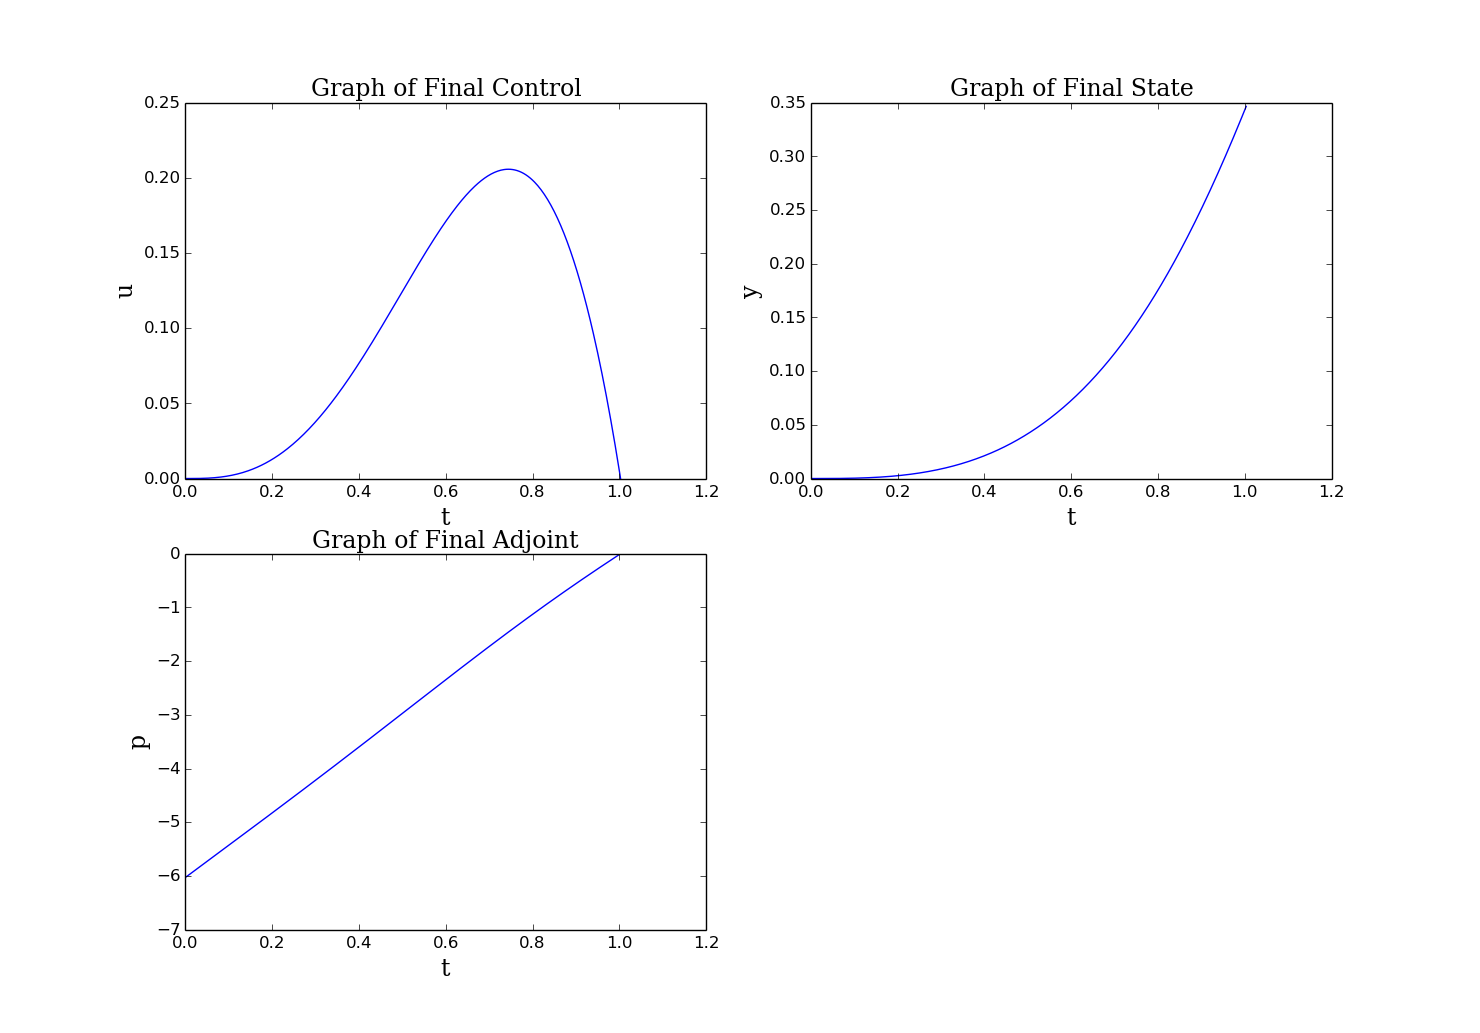
\includegraphics[scale=0.3]{u.png}
\caption{Final Iterations}
\label{final}
\end{figure}
The final control resembles a function of the shape $at \sin(bt)$ which would be an indicator
to why the second starting point resulted in fewer iterations. On the other hand, the second starting point corresponds
to a much more complicated graph who attains much higher values. This might suggest that this starting point is less suited, which is not on par with the results. The final state looks like
a hyperbolic function while the final adjoint looks linear.
\end{document}
